\documentclass{article}
\usepackage[utf8]{inputenc}
\usepackage{amsmath}
\usepackage{amsfonts}
\usepackage{graphicx}
\usepackage{multicol}
\usepackage{float}
\usepackage{cite}
\usepackage{url}

\begin{document}
	\begin{titlepage}
		\begin{center}
			{\huge\textbf{Instituto Politécnico Nacional}}\\
			\vspace{7mm}
			{\huge\textbf{Escuela Superior de Cómputo}}\\			
			\begin{figure}[h]
				\centering
				
\includegraphics[height = 6cm]{logoEscom.png}
			\end{figure}	
			\vspace{1cm}
			{\huge\textbf{Programa 3: Tablero}}
			\par\vspace{2cm}
			\large\textbf{Autor: Colín Ramiro Joel}
			\par\vspace{1cm}
			{\large\textbf{Materia: Teoría de la Computación}}
			\par\vspace{1cm}
			{\large\textbf{Grupo: 4CM2}}
			\par\vspace{1cm}
			{\large\textbf{Profesor: Juarez Martínez Gemaro}}
			\par\vspace{1cm}
			{\large\textbf{Fecha de entrega: {\huge{12 de Octubre 2021}}}}
			\par\vspace{3cm}
		\end{center}
	\end{titlepage}
	
	
	
	
	\section*{Introduction}
	\section*{Instrucciones}
	Elaborar un programa para realizar movimientos ortogonales y diagonales en un tablero de ajedrez de 4x4 con una pieza. Los movimientos y las reglas están explicadas en las láminas del curso de Stanford.
	Adicionalmente, el programa debe de contar con las siguientes características:
	\begin{enumerate}
		\item Debe de correr en modo automático y forma manual.	
		\item El usuario podrá introducir la cadena de movimientos o generarla aleatoriamente, con un máximo de 100 caracteres para el caso aleatorio. Si se escoge el modo manual las cadenas generadas no deben ser mayores a 20 movimientos.
		\item El autómata que se va a programar es el NFA.
		\item El estado inicial es el estado 1 y el final el estado 16.
		\item Una vez definida la cadena de movimientos para una pieza, se deben generar los archivos de todos los movimientos posibles y generar otro archivo con todos los movimientos ganadores.
		\item Dibujar el tablero y mostrar los movimientos de dos jugadas seleccionadas aleatoriamente del archivo de movimientos ganadoras. Para el caso de la animación pueden intentar poner la pieza del rey con bitmap o dibujar un circulo dentro del cuadrado, para posteriormente despintar y pintar el círculo, de manera que parezca que se mueve. Sugerencia: para dibujar el tablero utilizar la función de la librería gráfica que refiera un cuadrado y aplicar un fill para ponerle el color.
		\item En el reporte debe de estar también el código de la implementación.
	\end{enumerate}
	\section*{Desarrollo}
	Este programa se realizó en un solo archivo a diferencia del programa anterior. El programa solicitaba que tuviese la opción de correr manual y automáticamente, asi que hicimos un tipo de menú para que el usuario escojiese la opción.
	Támbien con el NFA el programa deberia de tomar la cadena ya sea propuesta por el usuario o generada automáticamente por el programa y validar dicha cadena, la cual si resulta ganadora, se debia de escribir en un archivo txt llamado "Ganadoras.txt" y todas las demás en otro archivo txt llamado "Todas.txt"

	
	
	\section*{Capturas del Funcionamiento}
	Primordialmente se creó una especie de menú para que el usuario introdujese la opción requerida ya sea que el programa funcione manual o automaticamente.
	
	\centering
	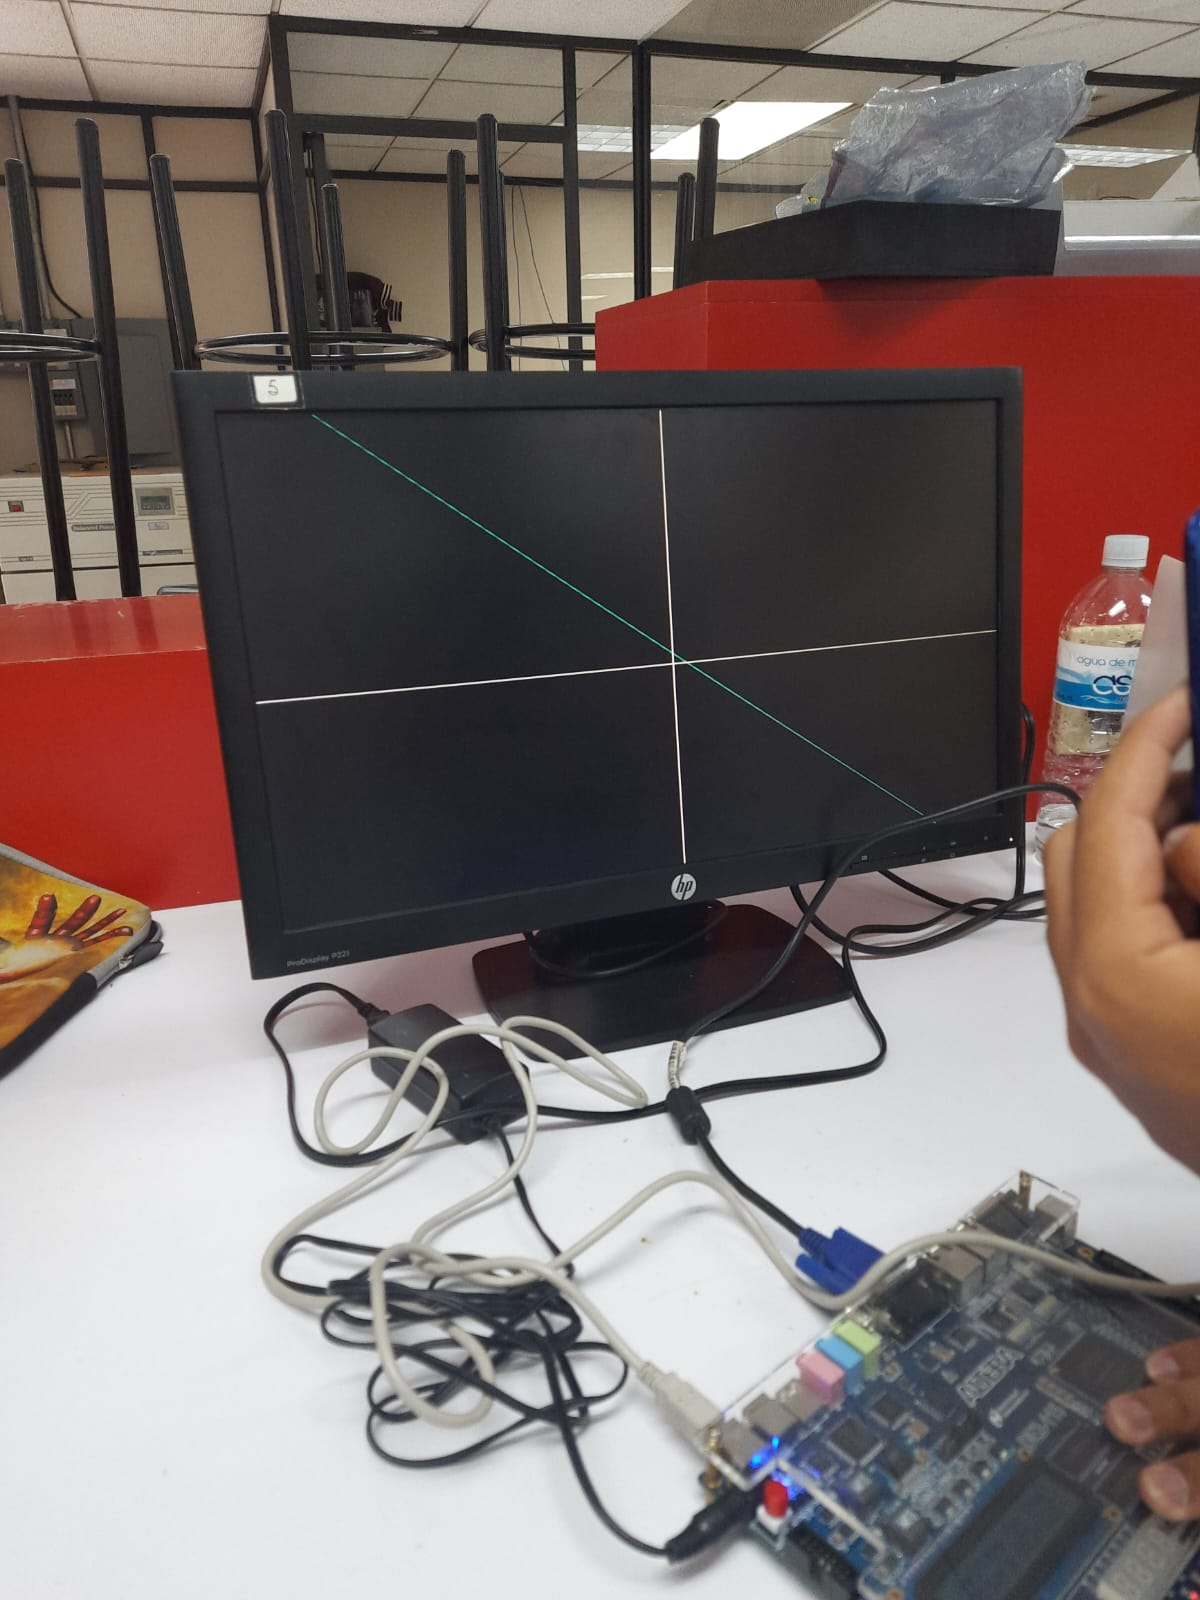
\includegraphics[width=5cm]{1.jpg}
	\includegraphics[width=5cm]{11.jpg}
	
	
	Y finalmente se crea el tablero en una ventana emergente via Python.
	\includegraphics[width=5cm]{tab.jpg}


	\section*{Código}
	La elaboración de este programa si resultó un código un poco largo, se adjuntan las capturas.
	
	\centering
	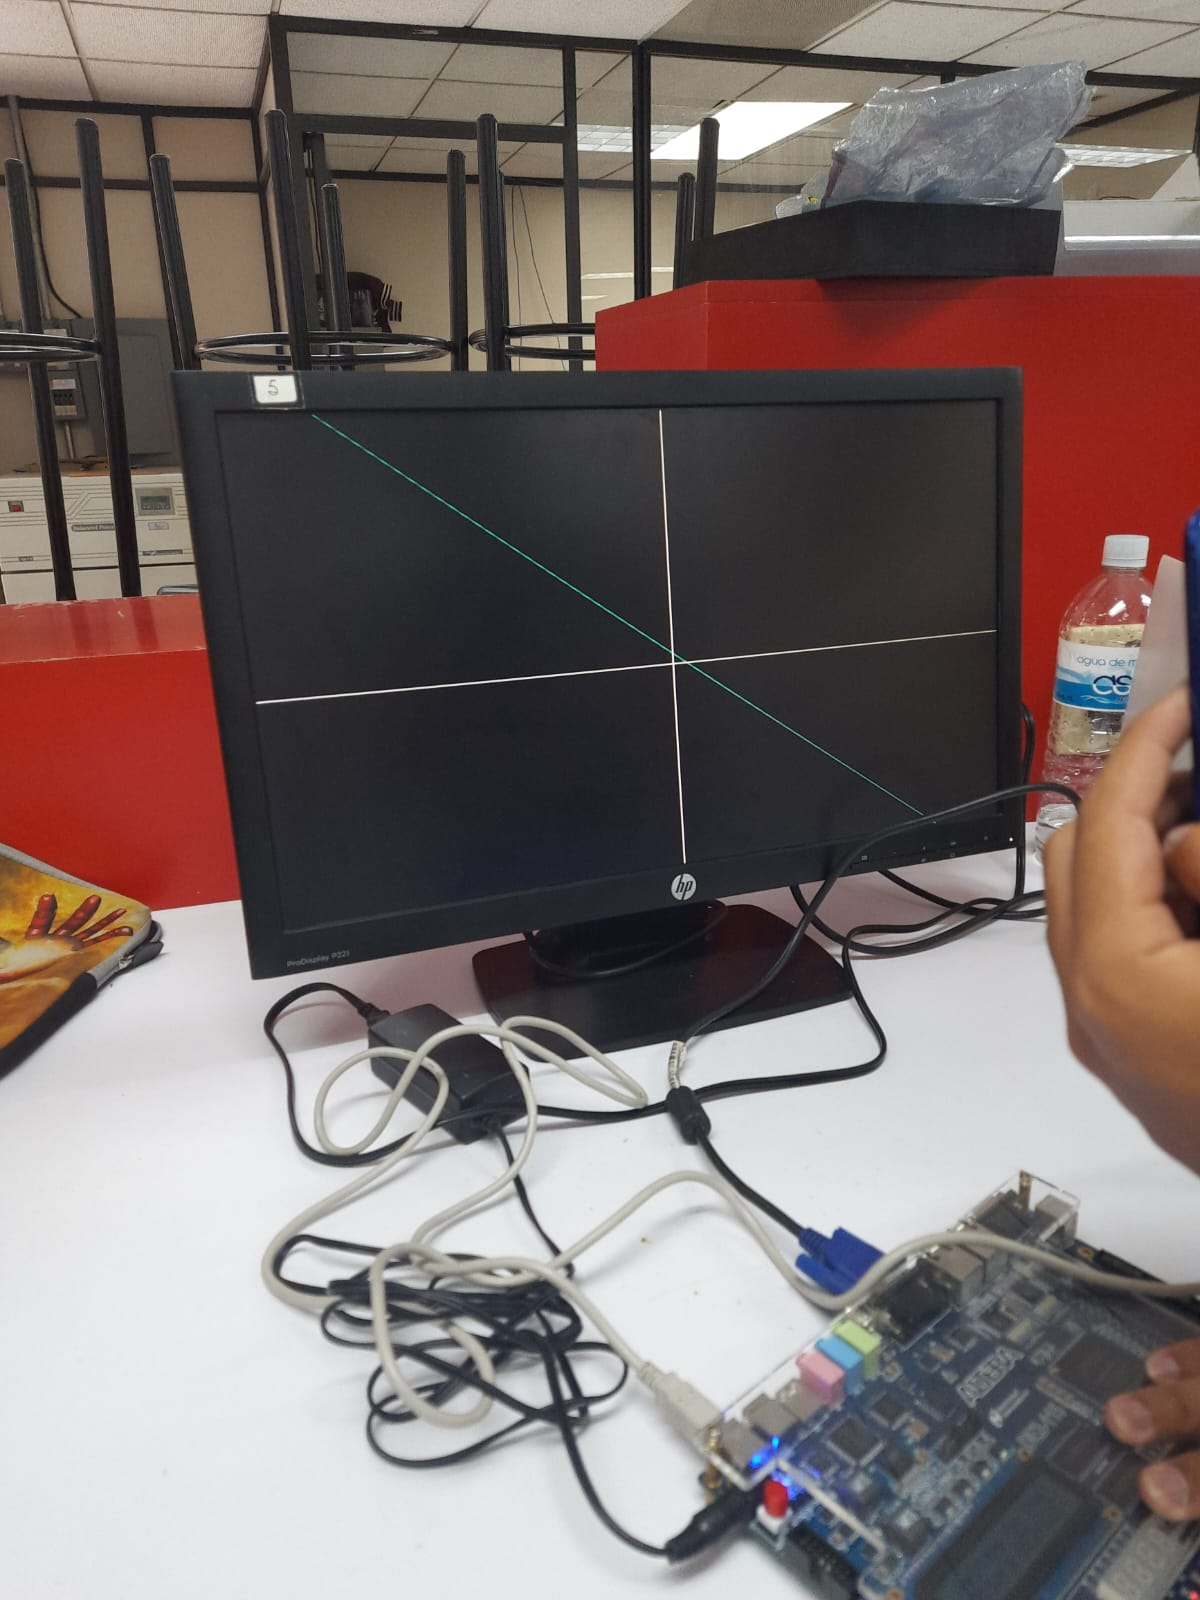
\includegraphics[width=5cm]{1.jpg}
	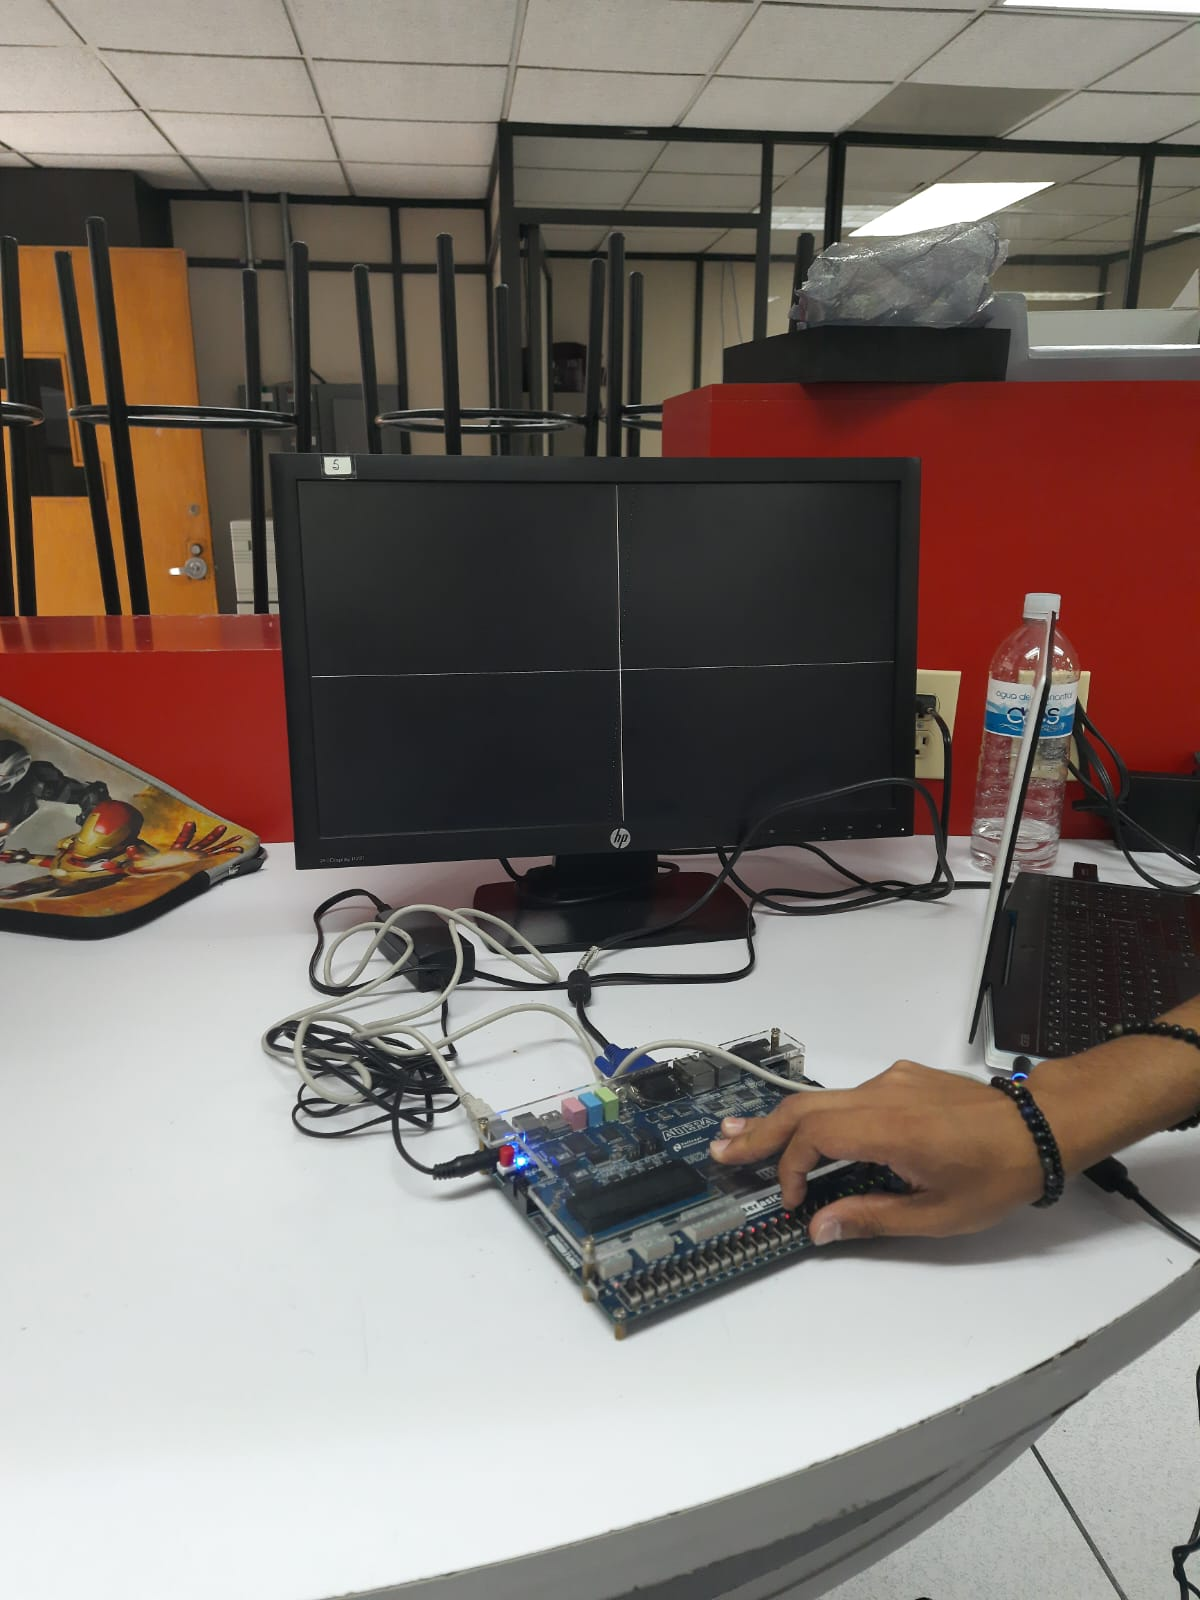
\includegraphics[width=5cm]{2.jpg}
	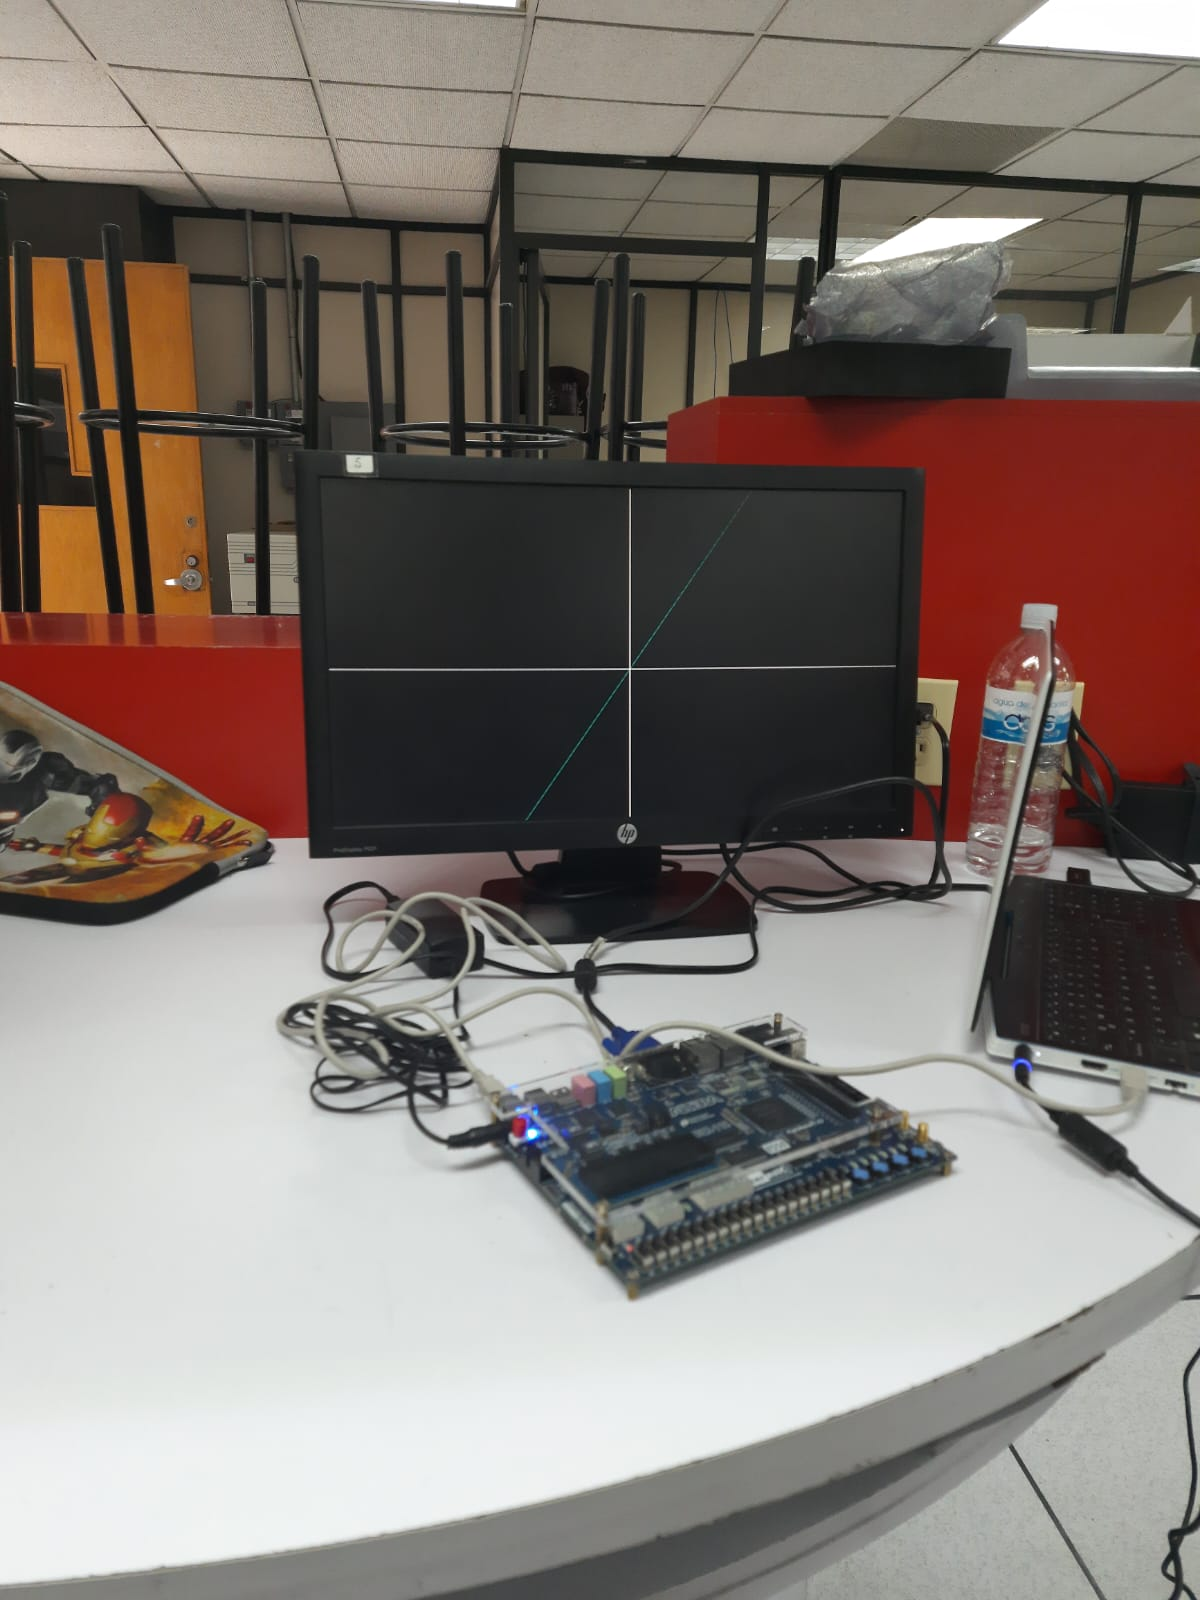
\includegraphics[width=5cm]{3.jpg}
	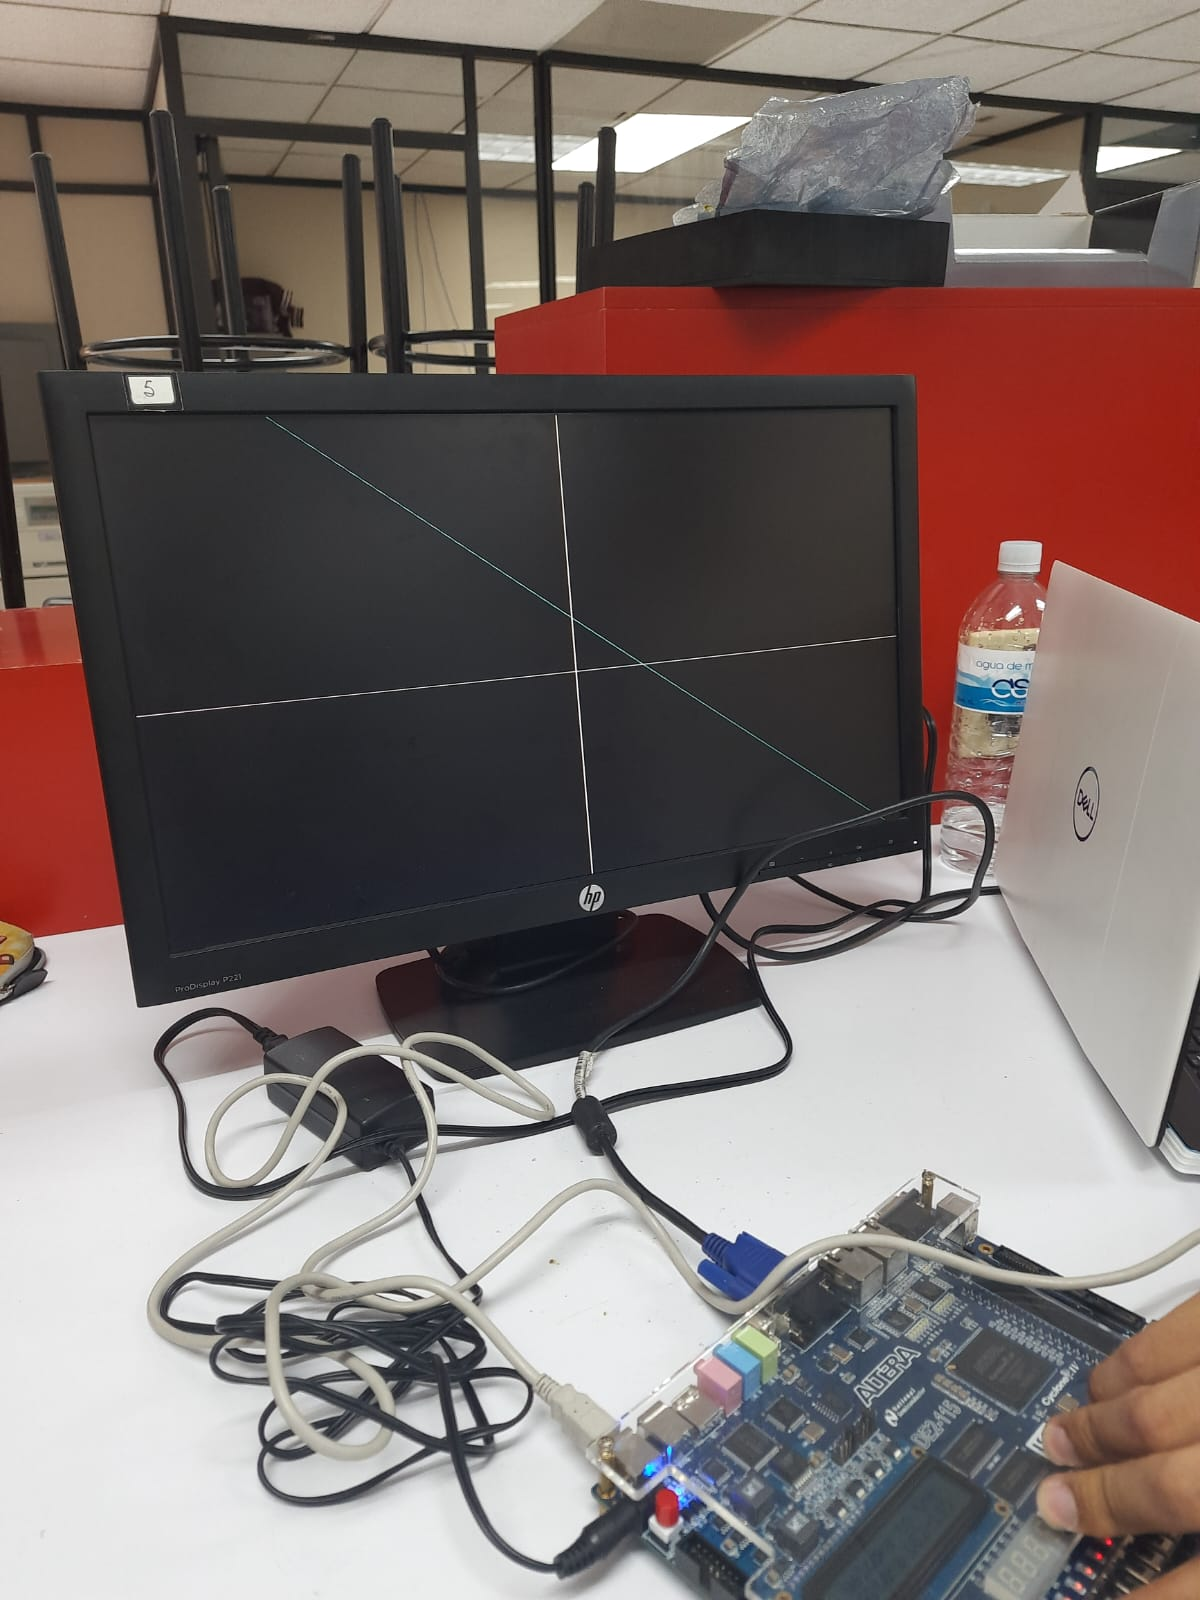
\includegraphics[width=5cm]{4.jpg}
	\includegraphics[width=5cm]{5.jpg}
	\includegraphics[width=5cm]{6.jpg}
	\includegraphics[width=5cm]{7.jpg}
	\includegraphics[width=5cm]{8.jpg}
	\includegraphics[width=5cm]{9.jpg}
	
	
	
	

	
\end{document}